%!TeX root=../wowtop.tex

\ArtChapter[What We Saw from the Ruined House]{19head}

\lettrine[lines=4,findent=2pt]{A}{fter} eating we crept back to the scullery, and there I must have dozed again, for when presently I looked round I was alone. The thudding vibration continued with wearisome persistence. I whispered for the curate several times, and at last felt my way to the door of the kitchen. It was still daylight, and I perceived him across the room, lying against the triangular hole that looked out upon the Martians. His shoulders were hunched, so that his head was hidden from me.

I could hear a number of noises almost like those in an engine shed; and the place rocked with that beating thud. Through the aperture in the wall I could see the top of a tree touched with gold and the warm blue of a tranquil evening sky. For a minute or so I remained watching the curate, and then I advanced, crouching and stepping with extreme care amid the broken crockery that littered the floor.

I touched the curate's leg, and he started so violently that a mass of plaster went sliding down outside and fell with a loud impact. I gripped his arm, fearing he might cry out, and for a long time we crouched motionless. Then I turned to see how much of our rampart remained. The detachment of the plaster had left a vertical slit open in the debris, and by raising myself cautiously across a beam I was able to see out of this gap into what had been overnight a quiet suburban roadway. Vast, indeed, was the change that we beheld.

The fifth cylinder must have fallen right into the midst of the house we had first visited. The building had vanished, completely smashed, pulverised, and dispersed by the blow. The cylinder lay now far beneath the original foundations—deep in a hole, already vastly larger than the pit I had looked into at Woking. The earth all round it had splashed under that tremendous impact—»splashed« is the only word—and lay in heaped piles that hid the masses of the adjacent houses. It had behaved exactly like mud under the violent blow of a hammer. Our house had collapsed backward; the front portion, even on the ground floor, had been destroyed completely; by a chance the kitchen and scullery had escaped, and stood buried now under soil and ruins, closed in by tons of earth on every side save towards the cylinder. Over that aspect we hung now on the very edge of the great circular pit the Martians were engaged in making. The heavy beating sound was evidently just behind us, and ever and again a bright green vapour drove up like a veil across our peephole.

\begin{figure}[tbp]
\centering
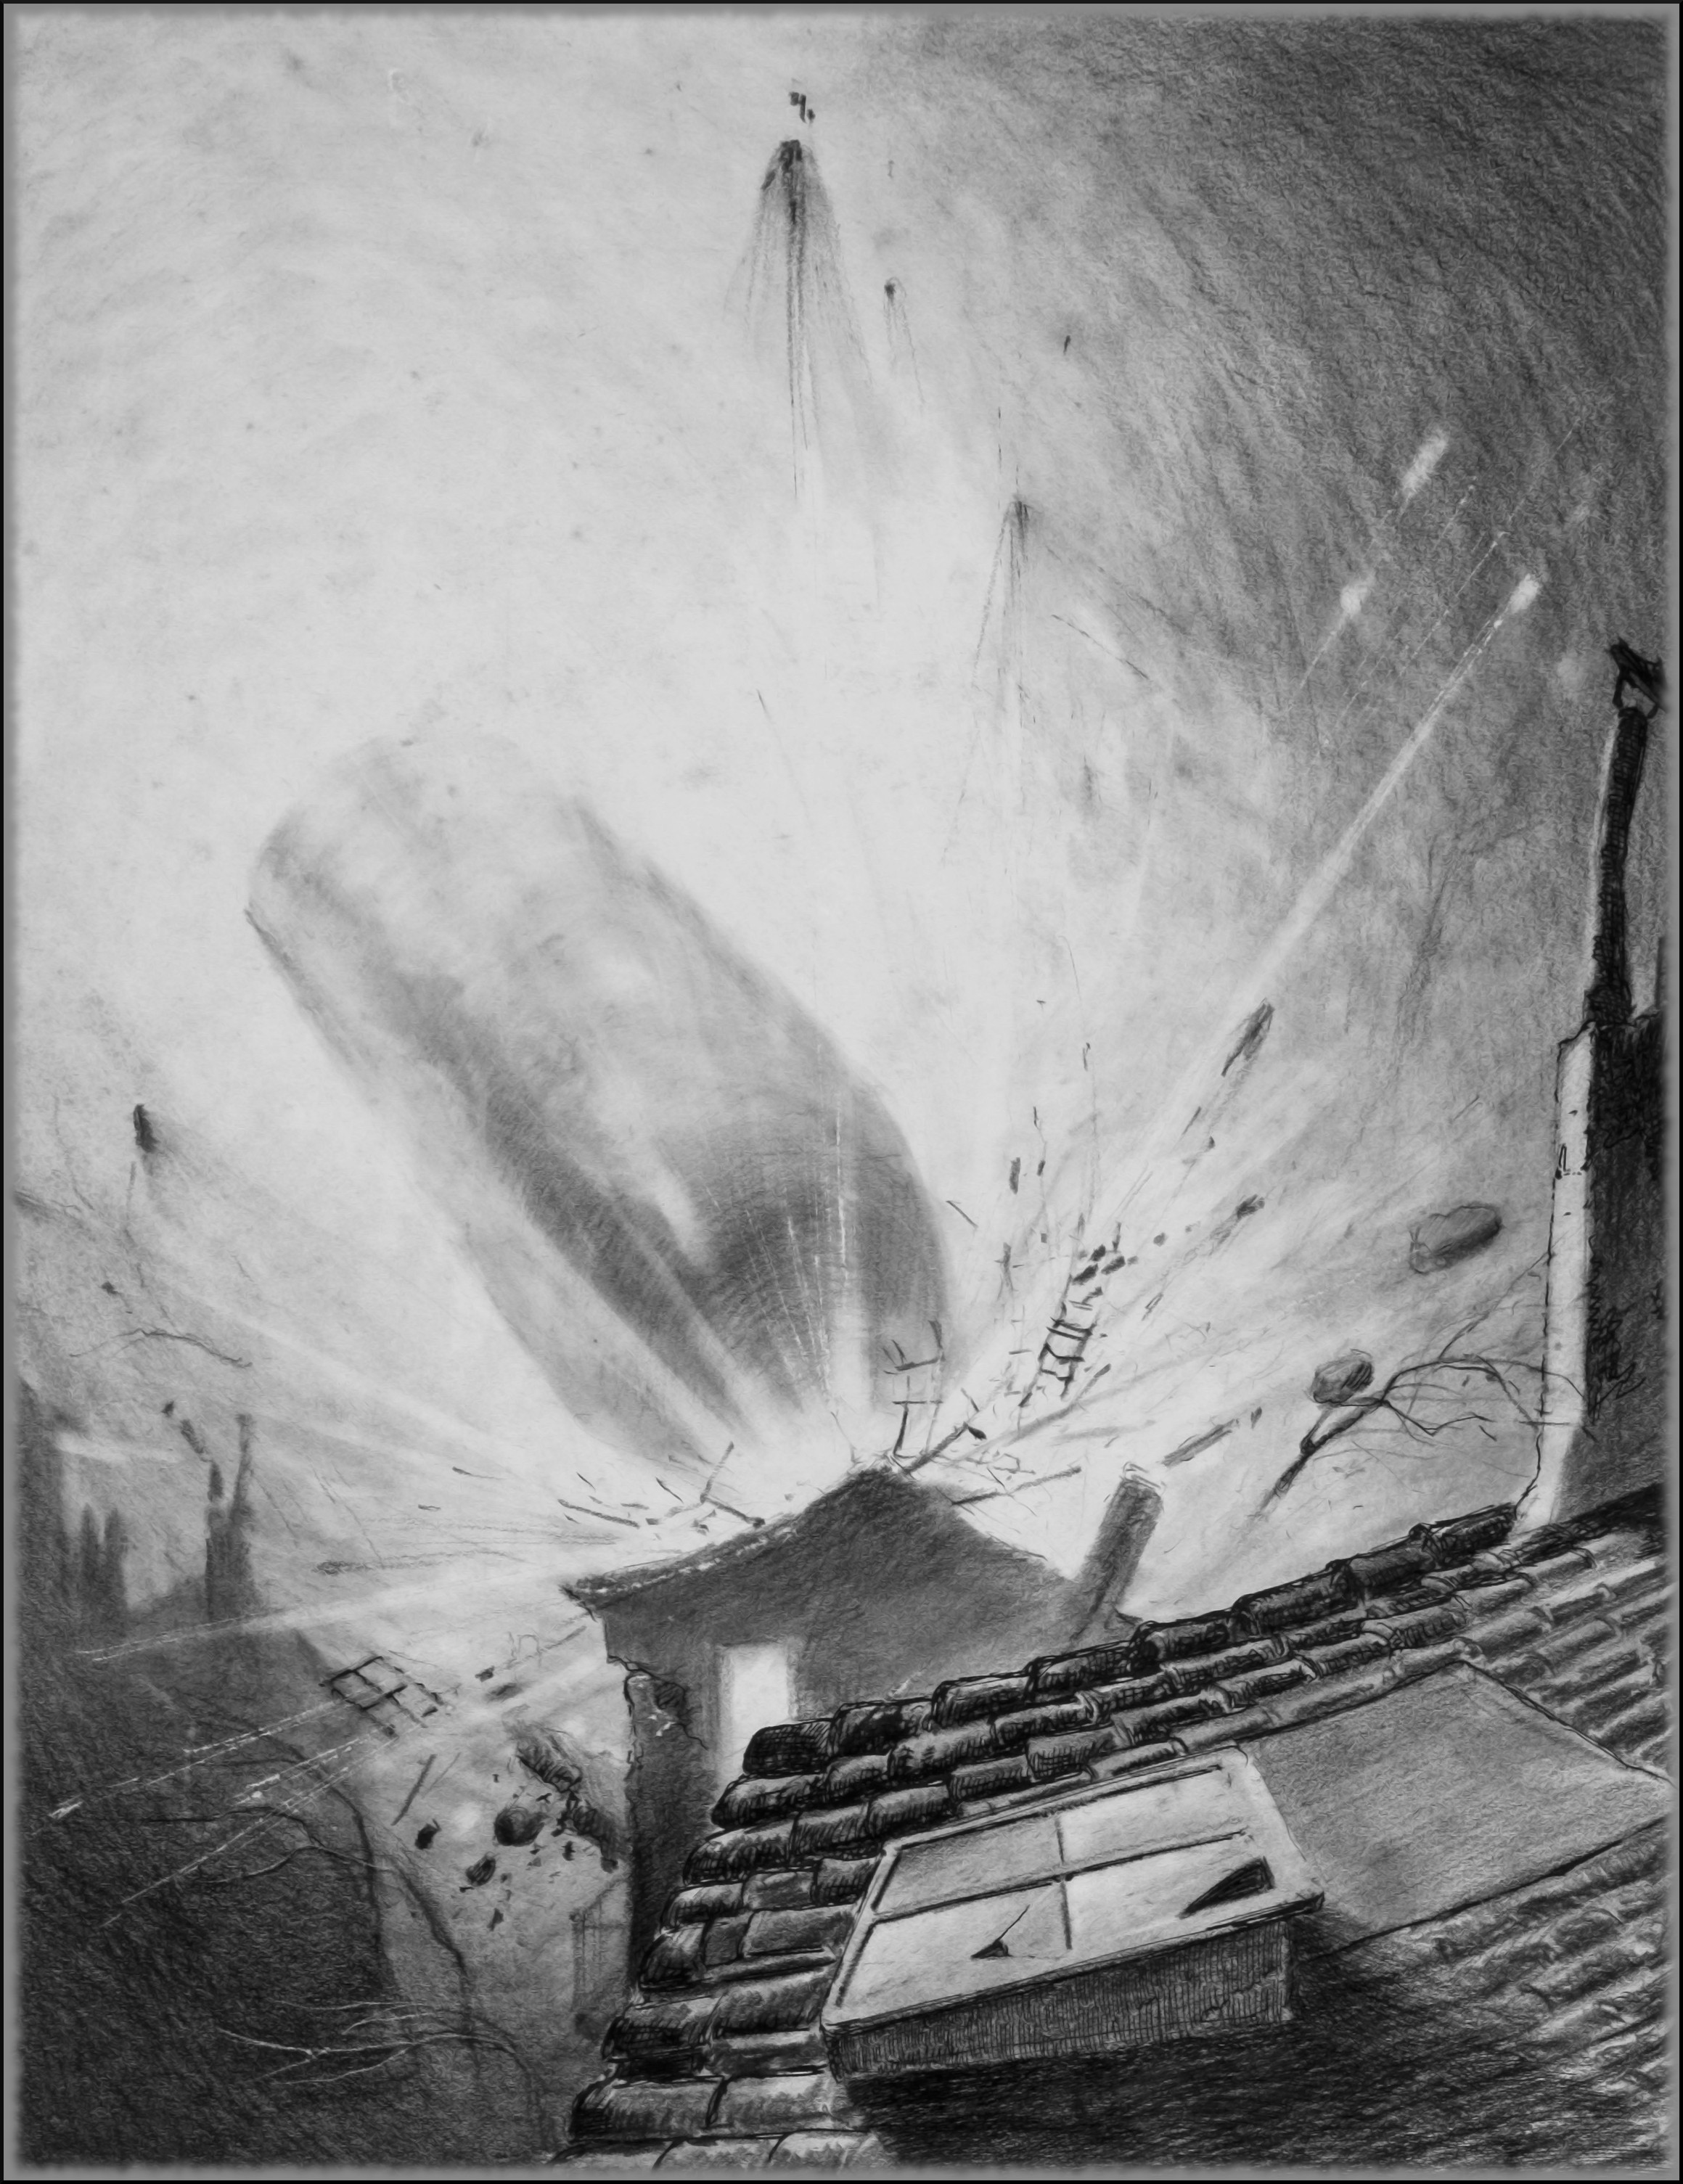
\includegraphics[width=\linewidth]{19fifthcylinder}
\caption[The building was completely smashed by the blow]{The building had vanished, completely smashed, pulverised, and dispersed by the blow}
\end{figure}

The cylinder was already opened in the centre of the pit, and on the farther edge of the pit, amid the smashed and gravel-heaped shrubbery, one of the great fighting-machines, deserted by its occupant, stood stiff and tall against the evening sky. At first I scarcely noticed the pit and the cylinder, although it has been convenient to describe them first, on account of the extraordinary glittering mechanism I saw busy in the excavation, and on account of the strange creatures that were crawling slowly and painfully across the heaped mould near it.


\begin{figure}[tbp]
\centering

\includegraphics[width=\linewidth]{19eveningsky}
\caption[Tall against the evening sky]{One of the great fighting-machines stood stiff and tall against the evening sky}
\end{figure}

The mechanism it certainly was that held my attention first. It was one of those complicated fabrics that have since been called handling-machines, and the study of which has already given such an enormous impetus to terrestrial invention. As it dawned upon me first, it presented a sort of metallic spider with five jointed, agile legs, and with an extraordinary number of jointed levers, bars, and reaching and clutching tentacles about its body. Most of its arms were retracted, but with three long tentacles it was fishing out a number of rods, plates, and bars which lined the covering and apparently strengthened the walls of the cylinder. These, as it extracted them, were lifted out and deposited upon a level surface of earth behind it.

Its motion was so swift, complex, and perfect that at first I did not see it as a machine, in spite of its metallic glitter. The fighting-machines were coordinated and animated to an extraordinary pitch, but nothing to compare with this. People who have never seen these structures, and have only the ill-imagined efforts of artists or the imperfect descriptions of such eye-witnesses as myself to go upon, scarcely realise that living quality.

\begin{figure}[tbp]
\centering

\includegraphics[width=\linewidth]{19spider}
\caption[At first I did not see it as a machine]{Its motion was so swift, complex, and perfect that at first I did not see it as a machine}
\end{figure}

I recall particularly the illustration of one of the first pamphlets to give a consecutive account of the war. The artist had evidently made a hasty study of one of the fighting-machines, and there his knowledge ended. He presented them as tilted, stiff tripods, without either flexibility or subtlety, and with an altogether misleading monotony of effect. The pamphlet containing these renderings had a considerable vogue, and I mention them here simply to warn the reader against the impression they may have created. They were no more like the Martians I saw in action than a Dutch doll is like a human being. To my mind, the pamphlet would have been much better without them.

At first, I say, the handling-machine did not impress me as a machine, but as a crablike creature with a glittering integument, the controlling Martian whose delicate tentacles actuated its movements seeming to be simply the equivalent of the crab's cerebral portion. But then I perceived the resemblance of its grey-brown, shiny, leathery integument to that of the other sprawling bodies beyond, and the true nature of this dexterous workman dawned upon me. With that realisation my interest shifted to those other creatures, the real Martians. Already I had had a transient impression of these, and the first nausea no longer obscured my observation. Moreover, I was concealed and motionless, and under no urgency of action.

%\begin{figure}[tb!]
%\centering
%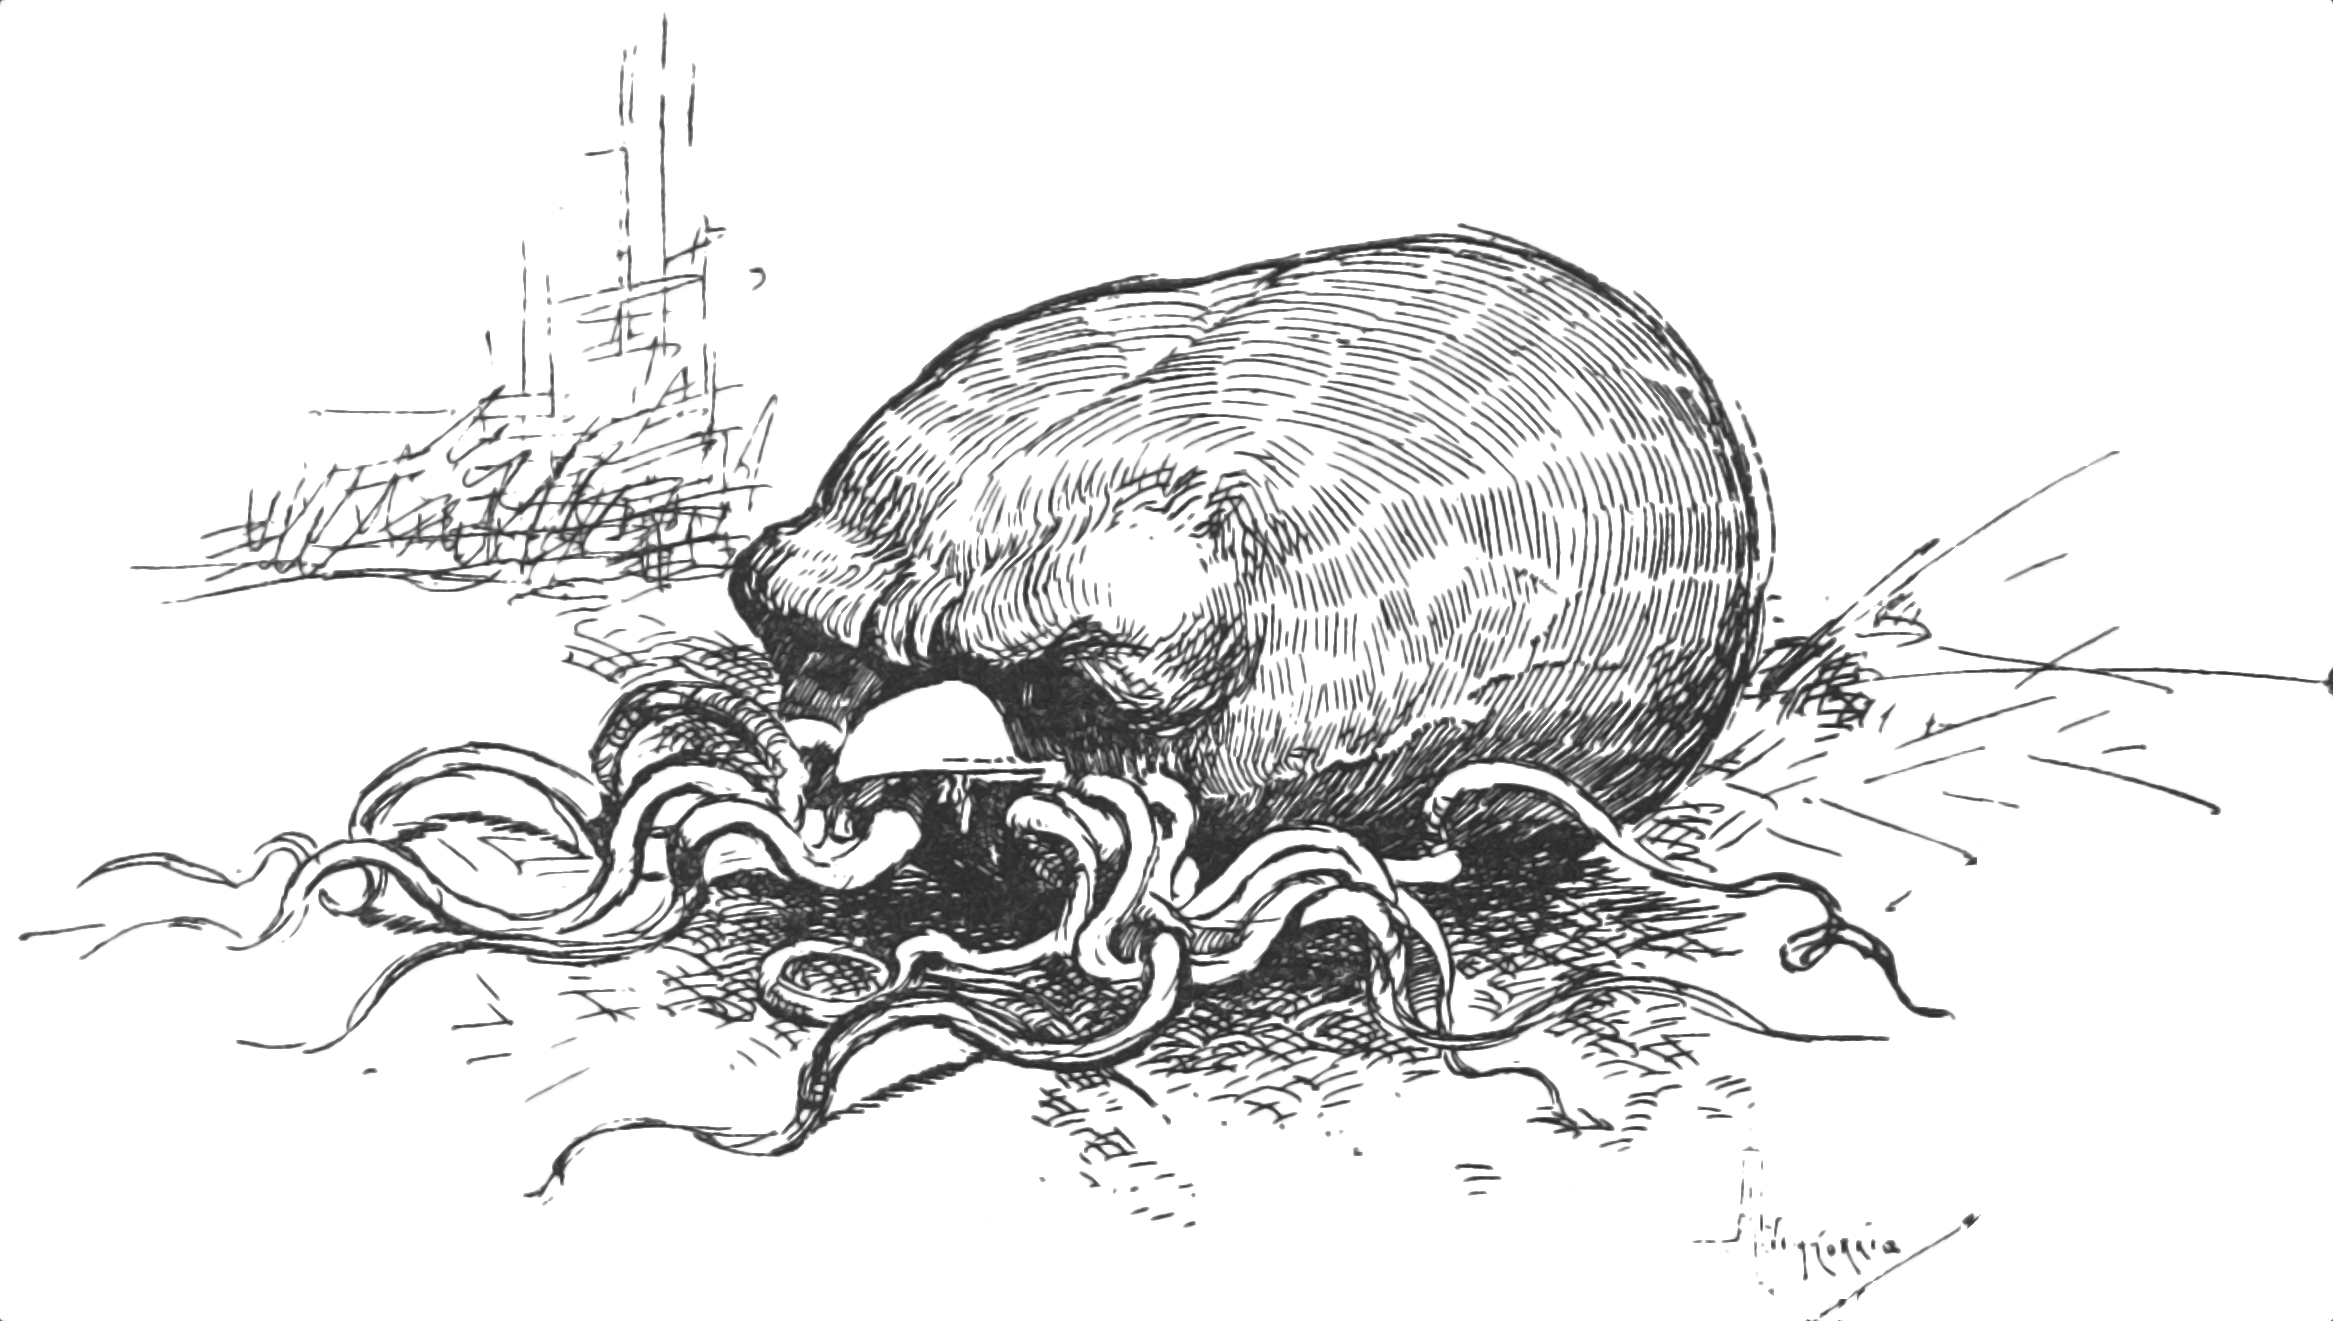
\includegraphics[width=\textwidth]{19biggianthead}
%\end{figure}

\begin{wrapfigure}{O}{0.5\textwidth}
\centering
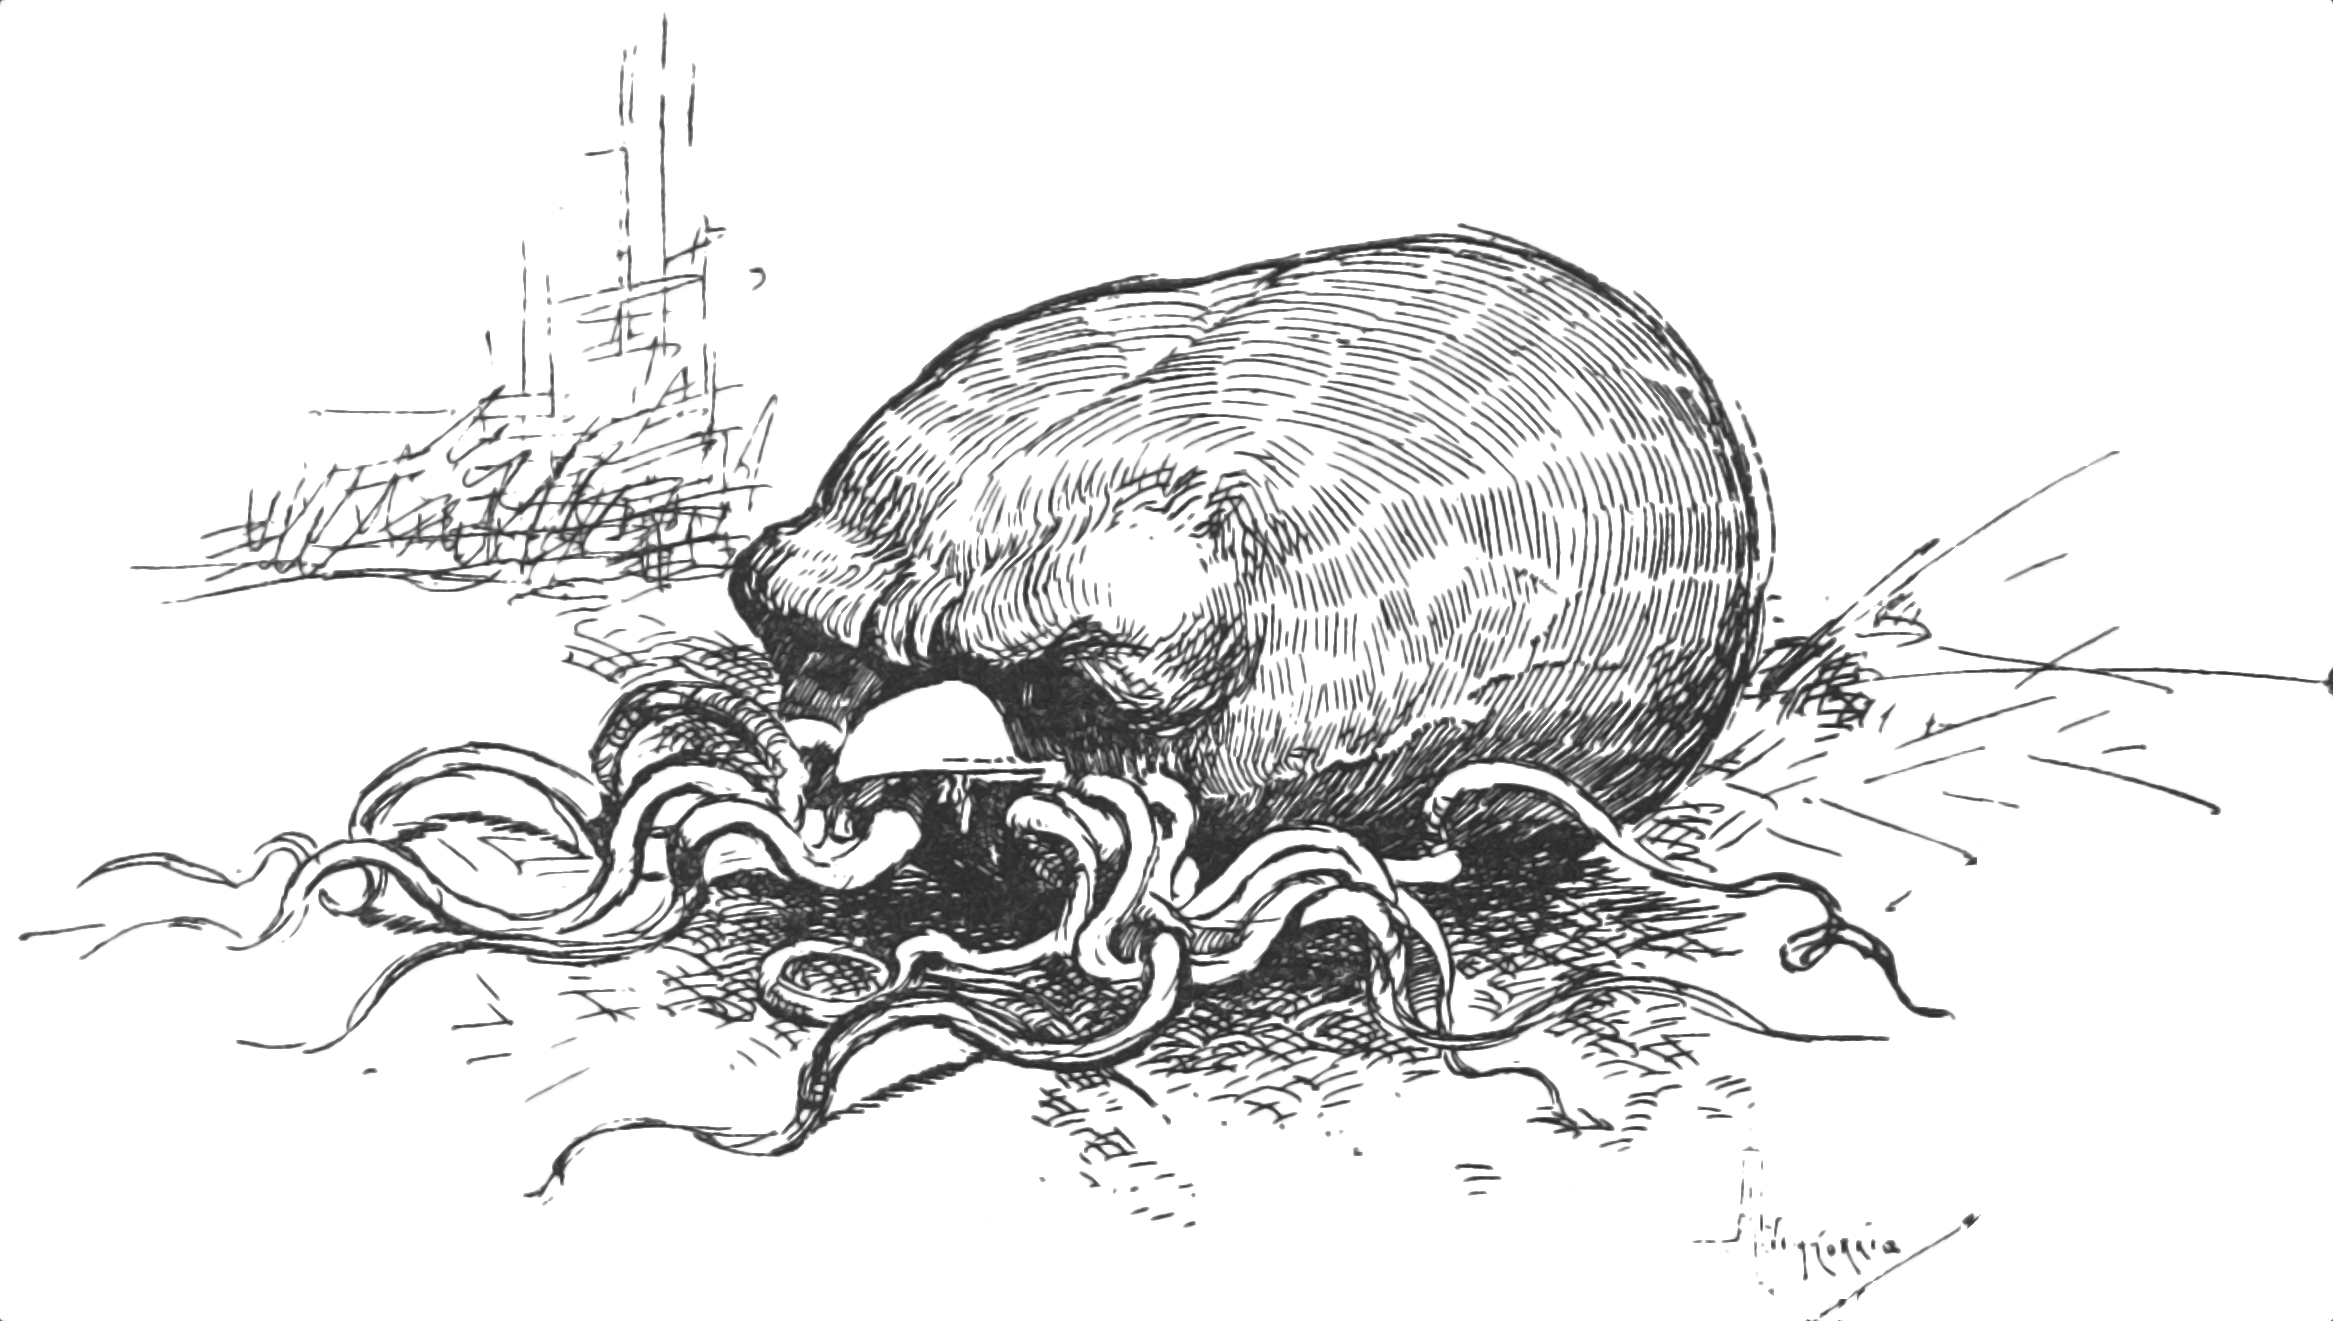
\includegraphics[width=0.5\textwidth]{19biggianthead}
\end{wrapfigure}

They were, I now saw, the most unearthly creatures it is possible to conceive. They were huge round bodies—or, rather, heads—about four feet in diameter, each body having in front of it a face. This face had no nostrils—indeed, the Martians do not seem to have had any sense of smell, but it had a pair of very large dark-coloured eyes, and just beneath this a kind of fleshy beak. In the back of this head or body—I scarcely know how to speak of it—was the single tight tympanic surface, since known to be anatomically an ear, though it must have been almost useless in our dense air. In a group round the mouth were sixteen slender, almost whiplike tentacles, arranged in two bunches of eight each. These bunches have since been named rather aptly, by that distinguished anatomist, Professor Howes, the \textit{hands}. Even as I saw these Martians for the first time they seemed to be endeavouring to raise themselves on these hands, but of course, with the increased weight of terrestrial conditions, this was impossible. There is reason to suppose that on Mars they may have progressed upon them with some facility.

The internal anatomy, I may remark here, as dissection has since shown, was almost equally simple. The greater part of the structure was the brain, sending enormous nerves to the eyes, ear, and tactile tentacles. Besides this were the bulky lungs, into which the mouth opened, and the heart and its vessels. The pulmonary distress caused by the denser atmosphere and greater gravitational attraction was only too evident in the convulsive movements of the outer skin.

And this was the sum of the Martian organs. Strange as it may seem to a human being, all the complex apparatus of digestion, which makes up the bulk of our bodies, did not exist in the Martians. They were heads—merely heads. Entrails they had none. They did not eat, much less digest. Instead, they took the fresh, living blood of other creatures, and \textit{injected} it into their own veins. I have myself seen this being done, as I shall mention in its place. But, squeamish as I may seem, I cannot bring myself to describe what I could not endure even to continue watching. Let it suffice to say, blood obtained from a still living animal, in most cases from a human being, was run directly by means of a little pipette into the recipient canal\textellipsis

The bare idea of this is no doubt horribly repulsive to us, but at the same time I think that we should remember how repulsive our carnivorous habits would seem to an intelligent rabbit.

The physiological advantages of the practice of injection are undeniable, if one thinks of the tremendous waste of human time and energy occasioned by eating and the digestive process. Our bodies are half made up of glands and tubes and organs, occupied in turning heterogeneous food into blood. The digestive processes and their reaction upon the nervous system sap our strength and colour our minds. Men go happy or miserable as they have healthy or unhealthy livers, or sound gastric glands. But the Martians were lifted above all these organic fluctuations of mood and emotion.

\begin{wrapfigure}{O}{0.4\textwidth}
\centering

\includegraphics[width=0.4\textwidth]{19almightytallest}
\end{wrapfigure}

Their undeniable preference for men as their source of nourishment is partly explained by the nature of the remains of the victims they had brought with them as provisions from Mars. These creatures, to judge from the shrivelled remains that have fallen into human hands, were bipeds with flimsy, silicious skeletons (almost like those of the silicious sponges) and feeble musculature, standing about six feet high and having round, erect heads, and large eyes in flinty sockets. Two or three of these seem to have been brought in each cylinder, and all were killed before earth was reached. It was just as well for them, for the mere attempt to stand upright upon our planet would have broken every bone in their bodies.

And while I am engaged in this description, I may add in this place certain further details which, although they were not all evident to us at the time, will enable the reader who is unacquainted with them to form a clearer picture of these offensive creatures.

In three other points their physiology differed strangely from ours. Their organisms did not sleep, any more than the heart of man sleeps. Since they had no extensive muscular mechanism to recuperate, that periodical extinction was unknown to them. They had little or no sense of fatigue, it would seem. On earth they could never have moved without effort, yet even to the last they kept in action. In twenty-four hours they did twenty-four hours of work, as even on earth is perhaps the case with the ants.

In the next place, wonderful as it seems in a sexual world, the Martians were absolutely without sex, and therefore without any of the tumultuous emotions that arise from that difference among men. A young Martian, there can now be no dispute, was really born upon earth during the war, and it was found attached to its parent, partially \textit{budded} off, just as young lilybulbs bud off, or like the young animals in the fresh-water polyp.

In man, in all the higher terrestrial animals, such a method of increase has disappeared; but even on this earth it was certainly the primitive method. Among the lower animals, up even to those first cousins of the vertebrated animals, the Tunicates, the two processes occur side by side, but finally the sexual method superseded its competitor altogether. On Mars, however, just the reverse has apparently been the case.

%\begin{wrapfigure}{O}{0.6\textwidth}
%\centering
%
\includegraphics[width=0.6\textwidth]{19womancaptured}
%\end{wrapfigure}

\begin{figure}[tb!]
\centering

\includegraphics[width=\textwidth]{19womancaptured}
\end{figure}


It is worthy of remark that a certain speculative writer of quasi-scientific repute, writing long before the Martian invasion, did forecast for man a final structure not unlike the actual Martian condition. His prophecy, I remember, appeared in November or December, 1893, in a long-defunct publication, the \textit{Pall Mall Budget}, and I recall a caricature of it in a pre-Martian periodical called \textit{Punch}. He pointed out—writing in a foolish, facetious tone—that the perfection of mechanical appliances must ultimately supersede limbs; the perfection of chemical devices, digestion; that such organs as hair, external nose, teeth, ears, and chin were no longer essential parts of the human being, and that the tendency of natural selection would lie in the direction of their steady diminution through the coming ages. The brain alone remained a cardinal necessity. Only one other part of the body had a strong case for survival, and that was the hand, »teacher and agent of the brain.« While the rest of the body dwindled, the hands would grow larger.

There is many a true word written in jest, and here in the Martians we have beyond dispute the actual accomplishment of such a suppression of the animal side of the organism by the intelligence. To me it is quite credible that the Martians may be descended from beings not unlike ourselves, by a gradual development of brain and hands (the latter giving rise to the two bunches of delicate tentacles at last) at the expense of the rest of the body. Without the body the brain would, of course, become a mere selfish intelligence, without any of the emotional substratum of the human being.

The last salient point in which the systems of these creatures differed from ours was in what one might have thought a very trivial particular. Micro-organisms, which cause so much disease and pain on earth, have either never appeared upon Mars or Martian sanitary science eliminated them ages ago. A hundred diseases, all the fevers and contagions of human life, consumption, cancers, tumours and such morbidities, never enter the scheme of their life. And speaking of the differences between the life on Mars and terrestrial life, I may allude here to the curious suggestions of the red weed.

Apparently the vegetable kingdom in Mars, instead of having green for a dominant colour, is of a vivid blood-red tint. At any rate, the seeds which the Martians (intentionally or accidentally) brought with them gave rise in all cases to red-coloured growths. Only that known popularly as the red weed, however, gained any footing in competition with terrestrial forms. The red creeper was quite a transitory growth, and few people have seen it growing. For a time, however, the red weed grew with astonishing vigour and luxuriance. It spread up the sides of the pit by the third or fourth day of our imprisonment, and its cactus-like branches formed a carmine fringe to the edges of our triangular window. And afterwards I found it broadcast throughout the country, and especially wherever there was a stream of water.

\begin{wrapfigure}{O}{0.3\textwidth}
\centering
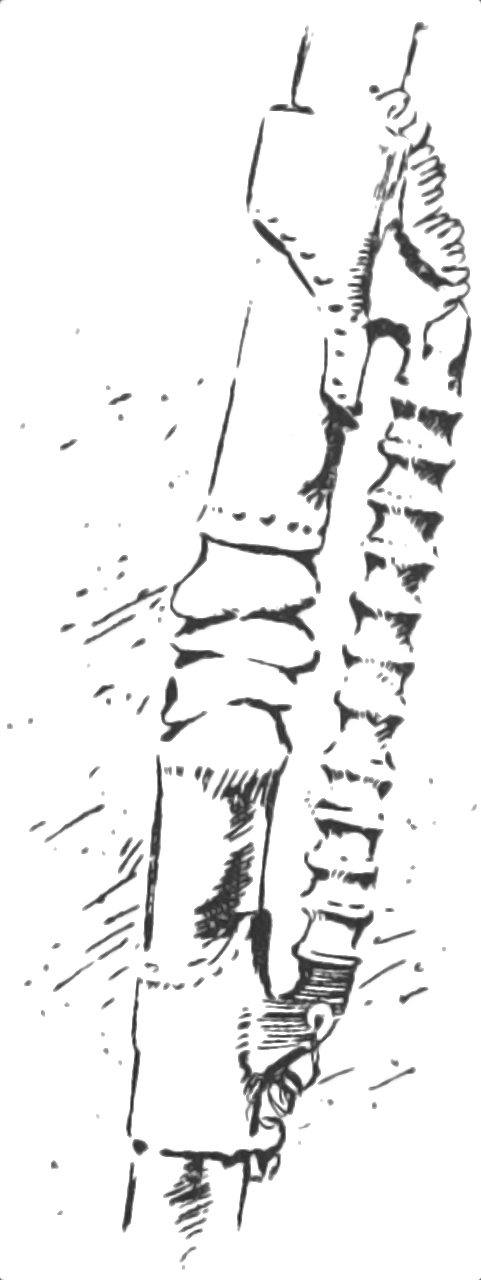
\includegraphics[width=0.3\textwidth]{19spinepipe}
\end{wrapfigure}

The Martians had what appears to have been an auditory organ, a single round drum at the back of the head-body, and eyes with a visual range not very different from ours except that, according to Philips, blue and violet were as black to them. It is commonly supposed that they communicated by sounds and tentacular gesticulations; this is asserted, for instance, in the able but hastily compiled pamphlet (written evidently by someone not an eye-witness of Martian actions) to which I have already alluded, and which, so far, has been the chief source of information concerning them. Now no surviving human being saw so much of the Martians in action as I did. I take no credit to myself for an accident, but the fact is so. And I assert that I watched them closely time after time, and that I have seen four, five, and (once) six of them sluggishly performing the most elaborately complicated operations together without either sound or gesture. Their peculiar hooting invariably preceded feeding; it had no modulation, and was, I believe, in no sense a signal, but merely the expiration of air preparatory to the suctional operation. I have a certain claim to at least an elementary knowledge of psychology, and in this matter I am convinced—as firmly as I am convinced of anything—that the Martians interchanged thoughts without any physical intermediation. And I have been convinced of this in spite of strong preconceptions. Before the Martian invasion, as an occasional reader here or there may remember, I had written with some little vehemence against the telepathic theory.





The Martians wore no clothing. Their conceptions of ornament and decorum were necessarily different from ours; and not only were they evidently much less sensible of changes of temperature than we are, but changes of pressure do not seem to have affected their health at all seriously. Yet though they wore no clothing, it was in the other artificial additions to their bodily resources that their great superiority over man lay. We men, with our bicycles and road-skates, our Lilienthal soaring-machines, our guns and sticks and so forth, are just in the beginning of the evolution that the Martians have worked out. They have become practically mere brains, wearing different bodies according to their needs just as men wear suits of clothes and take a bicycle in a hurry or an umbrella in the wet. And of their appliances, perhaps nothing is more wonderful to a man than the curious fact that what is the dominant feature of almost all human devices in mechanism is absent—the \textit{wheel} is absent; among all the things they brought to earth there is no trace or suggestion of their use of wheels. One would have at least expected it in locomotion. And in this connection it is curious to remark that even on this earth Nature has never hit upon the wheel, or has preferred other expedients to its development. And not only did the Martians either not know of (which is incredible), or abstain from, the wheel, but in their apparatus singularly little use is made of the fixed pivot or relatively fixed pivot, with circular motions thereabout confined to one plane. Almost all the joints of the machinery present a complicated system of sliding parts moving over small but beautifully curved friction bearings. And while upon this matter of detail, it is remarkable that the long leverages of their machines are in most cases actuated by a sort of sham musculature of the disks in an elastic sheath; these disks become polarised and drawn closely and powerfully together when traversed by a current of electricity. In this way the curious parallelism to animal motions, which was so striking and disturbing to the human beholder, was attained. Such quasi-muscles abounded in the crablike handling-machine which, on my first peeping out of the slit, I watched unpacking the cylinder. It seemed infinitely more alive than the actual Martians lying beyond it in the sunset light, panting, stirring ineffectual tentacles, and moving feebly after their vast journey across space.

While I was still watching their sluggish motions in the sunlight, and noting each strange detail of their form, the curate reminded me of his presence by pulling violently at my arm. I turned to a scowling face, and silent, eloquent lips. He wanted the slit, which permitted only one of us to peep through; and so I had to forego watching them for a time while he enjoyed that privilege.

When I looked again, the busy handling-machine had already put together several of the pieces of apparatus it had taken out of the cylinder into a shape having an unmistakable likeness to its own; and down on the left a busy little digging mechanism had come into view, emitting jets of green vapour and working its way round the pit, excavating and embanking in a methodical and discriminating manner. This it was which had caused the regular beating noise, and the rhythmic shocks that had kept our ruinous refuge quivering. It piped and whistled as it worked. So far as I could see, the thing was without a directing Martian at all.

\begin{a4}
	\begin{figure}[b!]
		\centering
		
\includegraphics[width=0.7\textwidth]{19tailpiece}
	\end{figure}
\end{a4}

\begin{letter}
	\begin{figure}[b!]
		\centering
		
\includegraphics[width=0.6\textwidth]{19tailpiece}
	\end{figure}
\end{letter}